\chapter{Forskningsdesign}
\label{ch:design}

I dette kapittelet presenteres og drøftes forskningsdesignet til studien.
Som nevnt tidligere, bygger rammeverket til forskningsprosessen på boken
\textit{Researching Information Systems and Computing} \citep{oates}.

\iffalse
I en forskningsartikkel er avsnittet om metode ofte det viktigste. Det samme gjelder metodekapitlet i en empirisk oppgave. Dette kan også være et vanskelig kapittel å skrive, fordi det ikke alltid er klart hvilken «jobb» det skal gjøre. Et metodekapittel skal ikke gjengi innholdet i fagets metodebøker. Dersom du har brukt intervju er det for eksempel ikke nødvendig å liste opp forskjellige typer forskningsintervju. Du trenger heller ikke redegjøre for forskjellene mellom kvantitative og kvalitative metoder, eller liste opp ulike typer validitet og reliabilitet.

Det du skal gjøre, er å vise hvordan dine valg av design og metode egner seg til å belyse/besvare ditt forskningsspørsmål, og hvilke vurderinger du har foretatt mht validitet (gyldighet) og reliabilitet (pålitelighet).’Show, don’t tell’ – vis leseren hva du gjorde, og forklar hvorfor. Da vil metodekapitlet sette de ulike delene av oppgaven i sammenheng, og det blir spennende å lese. I praksis betyr dette å demonstrere at du har forstått den praktiske betydningen av begrepene.

Et godt metodekapittel forteller hva du har gjort i din undersøkelse, og forklarer hvorfor. Hvordan samlet du inn data? Hva kan man forvente å finne ved å gjøre det på denne måten?
Hva var rammene? Hvilke avveininger måtte tas? Hva oppnår du ved å bruke denne metoden?
Vis hva du har gjort for å øke validiteten. Hva kan du si om reliabiliteten (påliteligheten) i datainnsamlingen? Hvordan vet du at du har undersøkt det du ønsket å undersøke? Hvilke slutninger kan trekkes på dette grunnlaget? Hvilke slutninger er sikre, og hvilke er mer tentative? Hvilken overføringsverdi har resultatene? Kan du generalisere – hvorfor, hvorfor ikke?
Svakheter og styrker ved metoden skal beskrives. Den ekstra gode oppgaven utmerker seg ved å forsvare sine valg og samtidig kritisere dem.

Formål
Produkter (bidrag/resultater)
Prosess
Deltakere
Paradigme
Presentasjon
\fi

\section{Forskningsspørsmål}
Som skrevet i kapittel \ref{ch:introduction}, er formålet med denne forskningen å undersøke hvordan ny teknologi basert
på \gls{iot}-skyløsninger kan brukes til avstandsoppfølging med prosjektet til Trondheim kommune som ramme:
\textbf{«\fs{}»}

Forskningsspørsmålene som ligger til grunn for denne masteroppgaven har gått igjennom en iterativ prosess i løpet av arbeidet
med oppgaven. Det vil si at intervjuene gjort med Trondheim kommune og arbeidet med den tekniske løsningen har påvirket
det prosjektet ønsker å undersøke nærmere. Alle forskningsstrategiene utdypes nærmere i delkapittel \ref{sec:forskningsstrategier}.

\subsection{Forskningsspørmål 1}
\textbf{\fs{1}}

Avstandsoppfølging er ganske nytt i Norge, og det foreligger ikke så mye informasjon om hvordan det gjøres ettersom
det i skrivende stund fortsatt er i testfasen i mange kommuner. Trondheim kommune vil bli brukt som et eksempel på hvordan avstandsoppfølging
gjøres i dag og hvilke planer de har for ny teknologi i tiden som kommer. Forskningsprosjektet vil finne ut hvilke utfordringer
kommunen har med avstandsoppfølging i dag og hvilke erfaringer de har gjort seg hittil.

For å belyse spørsmålet er forskningsløpet som i figur \ref{fig:oates_fs1}. Case-studie er hovedstrategien, og intervjuer og dokumenter
er datagenereringsmetodene. Intervjuene transkriberes der det er relevant og analyseres basert på temaer.

\begin{figure}
\centering
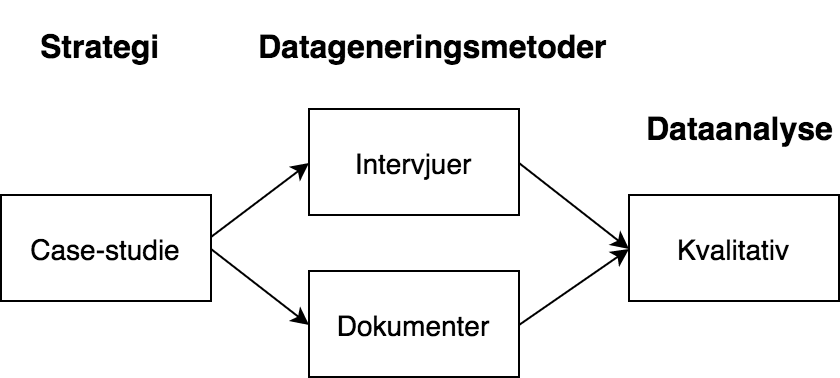
\includegraphics[width=0.65\textwidth]{fig/oates/fs1}
\caption{Forskningsstrategien til FS1}
\label{fig:oates_fs1}
\end{figure}

\subsection{Forskningsspørmål 2}
\textbf{\fs{2}}

Hovedstrategien er design og kreasjon, med intervjuer og dokumenter som datagenereringsmetode (figur \ref{fig:oates_fs2}). Ved å lage
et \textit{proof of concept} basert på eksisterende skyteknologi, er målet å finne en mulig arkitektur for teknologien. Case-studien av Trondheim
kommune hjelper til med å forstå brukskonteksten og kravene til en slik arkitektur og om denne arkitekturen kan hjelpe kommunen med de
utfordringene som blir belyst i case-studien.

Arkitektur er definert
som strukturen til klientsiden av applikasjonen, hvordan denne fungerer og snakker med sensorene rundt -- og på hvilken måte sensordataene sendes
fra klienten og behandles av en bakenforliggende serverløsning. Hele dette samspillet danner en mulig arkitektur for avstandsoppfølging.

\begin{figure}
\centering
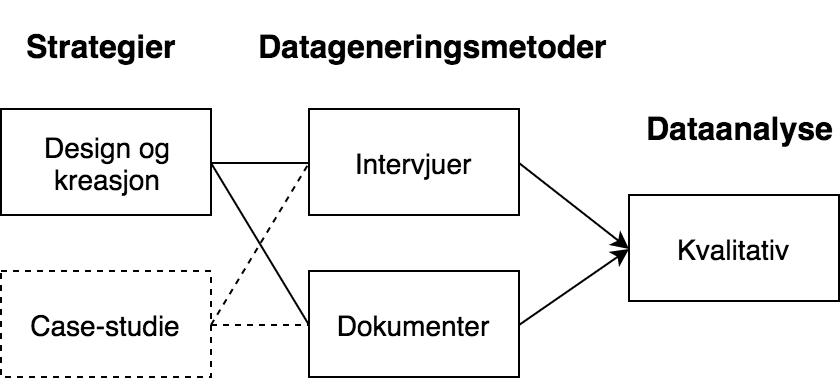
\includegraphics[width=0.65\textwidth]{fig/oates/fs2}
\caption{Forskningsstrategien til FS2}
\label{fig:oates_fs2}
\end{figure}
    
\subsection{Forskningsspørmål 3}
\textbf{\fs{3}}

Forskningsstrategien er å lage en frittstående løsning i form av et skytilkoblet pulsoksymeter og evaluere
denne løsningen med semistrukturerte intervjuer (figur \ref{fig:oates_fs3}).
 
Frittstående betyr at løsningen er helt plattformuavhengig og ikke basert på eksisterende plattformer som Android og iOS.
Domeneeksperter er definert som forskere, prosjektledere og ansatte innenfor velferdsteknologi og avstandsoppfølging.

\begin{figure}
\centering
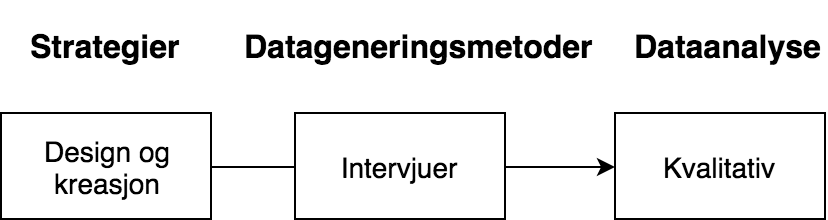
\includegraphics[width=0.65\textwidth]{fig/oates/fs3}
\caption{Forskningsstrategien til FS3}
\label{fig:oates_fs3}
\end{figure}

\subsection{Forskningsspørmål 4}
\textbf{\fs{4}}

Dette forskningsspørsmålet sammenstiller all data fra de andre forskningsspørsmålene. Det søker å finne ut hva implikasjonene
er for utviklingen av skybasert \gls{iot} for avstandsoppfølging gjennom en kvalitativ analyse og drøfting.
Figur \ref{fig:oates_fs4} oppsummerer hele forskningsløpet.

\begin{figure}
\centering
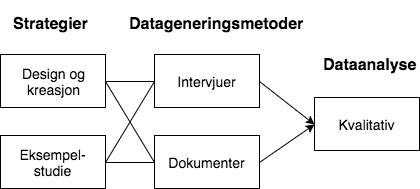
\includegraphics[width=0.65\textwidth]{fig/oates/fs4}
\caption{Forskningsstrategien til FS4}
\label{fig:oates_fs4}
\end{figure}

\section{Forskningsstrategier}
\label{sec:forskningsstrategier}
Dette delkapittelet drøfter og beskriver kort hva som skal skje i de forskningsstrategiene som er valgt.

\subsection{Design og kreasjon av et pulsoksymeter}
Artefakten i dette prosjektet er en høynivå prototype i form av et proof of concept, både på hardware- og softwaresiden.
Siden teknologiutforsking er et mål, vil
prototypen implementeres på et ganske høyt nivå, og ikke være en lavnivå papirprototype. Prototypen vil sammenlignes
med den eksisterende løsningen og vises fram til prosjektledere, ansatte og forskere innen velferdsteknologi.

Den industrielle utformingen av prototypen vektlegges ikke. Det er
ikke meningen at prototypen skal ut i produksjon slik som den er designet. En annen tilnærming kunne vært å vektlegge brukerperspektivet enda mer,
og gjennomføre flere runder med brukertester med helsepersonell og pasienter. Brukertester med pasienter ville medført krav om
riktig behandling av sensitive helseopplysninger og en godkjent søknad til Norsk senter for forskningsdata (NSD).

Brukersentrert utvikling er metodikken som brukes for design og kreasjon av prototypen. Filosofien bak å inkludere brukeren i hvert aspekt
av utviklingen er å fortere finne ut hva som ikke fungerer slik at en ikke maler seg inn i et hjørne. Case-studien av avstandsoppfølging
i Trondheim kommune hjelper til med å forstå konteksten pulsoksymeteret skal brukes i og hvordan det skal brukes, noe
som fører til at utviklingen av en prototype blir enklere.

\begin{minipage}{\linewidth}
Dette er design og kreasjon-strategien oppsummert:\newline

\begin{description}
  \item [Bevisstgjøring] Semistrukturert intervju med Trondheim kommune om velferdsteknologi og avstandsoppfølging. Kort bakgrunnkapittel
      om velferdsteknologi og avstandsoppfølging (kapittel \ref{ch:background}).
  \item [Forslag] En frittstående og skytilkoblet velferdsteknologiløsning der sensorene er innebygget vil fungere bedre
      eller like bra som eksisterende løsninger med nettbrett. Å basere seg på AWS IoT som skyplattform vil gjøre utviklingen enklere.
  \item [Utvikling] En prototype av et skytilkoblet pulsoksymeter med fingeravtrykksensor som autentiseringsmetode.
  \item [Evaluering] Semistrukturerte intervjuer med Trondheim kommune og SINTEF der prototypen vises fram.
  \item [Konklusjon] Baseres på alle de foregående stegene.
\end{description}
\end{minipage}

Hvordan evalueringen av prototypen med semistrukturerte intervjuer ble gjennomført er beskrevet i kapittel \ref{ch:evaluation1}.

\subsection{Case-studie: Avstandsoppfølging i Trondheim kommune}
Det er flere tilnærminger til avstandsoppfølging, og det er flere kommuner enn Trondheim som har pågående forsøk, blant annet
Sarpsborg og Oslo. Fordelen med å velge ut én kommune er at det belyser hvordan de har tilnærmet seg avstandsoppfølging
som helhet og forenkler datainnhentingen -- det er naturlig å velge ut Trondheim kommune siden det gjør at tilgangen på personer er bedre.

Målet med case-studien er å skjønne hvilke problemstillinger Trondheim kommune prøver å løse, hvordan de løser dem og hvilke
erfaringer de har gjort seg hittil. Dette vil påvirke den nye teknologien som bygges i dette forskningsprosjektet. Case-studien
vil gi en oversikt over tjenesten fra A til Å, fra hvordan brukerne blir rekruttert til hvordan de bruker løsningen hjemme.

Datageneringsmetoder i dette case-studiet er semistrukturerte intervjuer og dokumenter. Observasjon av hvordan pasientene bruker Trondheim kommunes løsning
kunne vært en god metode, men for å snevre inn omfanget og slippe å innhente tillatelser velges ikke denne metoden. Det hadde vært mer
aktuelt om case-studiet hadde vært den eneste hovedstrategien i prosjektet. Eksempler på dokumenter er all den informasjonen som finnes om
avstandsoppfølging på Internett og det Trondheim kommune har lagt ut selv. Helsedirektoratet og Datatilsynet
har også en rekke retningslinjer og råd som kommunene må og kan forholde seg til.

Hvordan de ulike intervjuene ble gjennomført og analysert er beskrevet i starten av kapittel \ref{ch:case}.

\section{Forskningsparadigme og forskningskvalitet}
Forskningsprosjektet inneholder kun kvalitative datagenereringsmetoder, og er dermed en form for kvalitativ forskning.
Det tar en interpretivistisk tilnærming til det som skal undersøkes. Det er flere måter å gjøre avstandsoppfølging på,
og det er ikke sikkert at en metode er bedre enn en annen.
Siden kun kvalitativ data analyseres, vil nødvendigvis forskerens subjektive holdninger påvirke drøftingen av forskningsspørsmålene.

Validitet og objektivitet må forstås på en annen måte i dette prosjektet enn om dette for eksempel hadde vært et
kvantitativt eksperiment. Lincoln og Guba foreslår, i følge \citet{oates},
at kriteriene for interpretivisme
heller skal være hvor stor tillit man kan ha til forskningen, gjennom begrepene bekreftbarhet, pålitelighet, troverdighet og overførbarhet.
Her handler bekreftbarhet og pålitelighet om hvorvidt studiet er godt nok beskrevet og dokumentert til at man skjønner hvordan det har
foregått og kan stole
på forskningsløpet. Forskning blir mer troverdig med flere forskjellige kilder til data og om man sjekker med kildene om man har
tolket data riktig. Dette diskuteres i delkapittel \ref{sec:validitet}.
